\documentclass[11pt]{texMemo-gibbons}
\usepackage[english]{babel}
\usepackage{graphicx}
\usepackage{blindtext}
\usepackage{amsmath,amssymb,units}
\usepackage{siunitx}
\usepackage[outdir=./]{epstopdf}
\usepackage{subfigure}
\memostudent{Ty Davis}
\memocourse{ECE 3210}
\memosubject{Lab 6, Aliasing}
\memodate{\today}
\logo{
\includegraphics[width=0.5\textwidth]{ece_horiz.pdf}}

\begin{document}
\maketitle

\section{Introduction}
\label{sec:introduction}

This will be a bit of a shorter lab where we study the
phenomenon of aliasing using a few techniques. We will
be producing sine wave signals and then sampling them 
at different rates to see the affect of sampling below
the Nyquist frequency.

\section{Theory}
\label{sec:theory}

A sine wave is produced with the following expression:

\[
  x(t) = A \sin (2\pi f_0 t + \phi)
\]

Sampling that frequency at a separate sampling frequency $f_s$ can be modeled
with this expression:

\[
  x[k] = A \sin \Big( 2\pi k \Big( \frac{f_0}{f_s} \Big)  + \phi \Big)
\]

With a sampling period $T$ where $T=\frac{1}{f_s}$ we can also show 
$x[k]$ with this:

\begin{equation}
  x[k] = A \sin ( 2\pi k T + \phi )
  \label{eq:sampling_sine}
\end{equation}

The other portion of this lab requires us to play a chirp signal
which is a signal that has a frequency that increases linearly
with time. It is shown by Eq.~\ref{eq:chirp}.

\begin{equation}
  c(t) = A \cos (\pi \mu t^2 + 2\pi f_1 + \phi) 
  \label{eq:chirp}
\end{equation}

\section{Results}
\label{sec:results}

When comparing the plots shown in Fig.~\ref{fig:low_freq_stem}
and Fig.~\ref{fig:high_freq_stem} we can see that the
stem plots appear very similar. This is due to aliasing.
The frequency of the signal is so close to the frequency
of the sample rate that the true waveform of the signal
is lost.

The only difference between the plots is that the sampled
higher frequency signal is 180 degrees out of phase
from the lower frequency signal.

When sampling the chirp signal shown by at different frequencies
we can hear different results. When sampling at a very
high frequency --- 32 kHz --- the chirp signal increased
linearly in frequency until the duration expired, but
when we sampled at a lower frequency --- 16 kHz ---
we heard something else. The tone got higher at the
same rate as the original tone, about half way through
the duration it suddenly started to get lower. Again,
when sampled at 8 kHz, the tone increased until just
1/4 of the duration, then decreased until it was too
low to hear. This was at just have the duration though,
and the pattern repeated again in the same fashion until
the entire duration expired.

The perceived tones approximately followed the pattern
shown in Fig.~\ref{fig:chirp_samples}.

\section{Discussion and Conclusions}
\label{sec:conclusions}

The aliasing phenomenon is demonstrated in Fig.~\ref{fig:aliasing}
where a higher-frequency signal and a lower frequency
signal intersect at every point where they are sampled.

This is why the signals shown in the Fig.~\ref{fig:low_freq_stem}
and Fig.~\ref{fig:high_freq_stem} sound identical when
sampled at that sample rate. Even though the frequency
of one signal is dramatically higher than the other,
when sampled they result in the same signal.

Fig.~\ref{fig:chirp_samples} shows that sampling at
a really high frequency is necessary to prevent the
high frequencies from being interpreted and transmitted
as lower frequencies. In the case of telephone communication,
this is impractical because a lot of data would be used
to store information about really high frequencies that
aren't necessary for common dialogue that occurs well below
1 kHz.

Because of this, and anti-aliasing filter, or low-pass
filter, is used on the signal before being sampled.
This essentially cuts off the entire right portion of
the graph in Fig.~\ref{fig:chirp_samples} and doesn't
disturb any of the input signal that we care about.



\clearpage

\begin{figure}
  \centering
  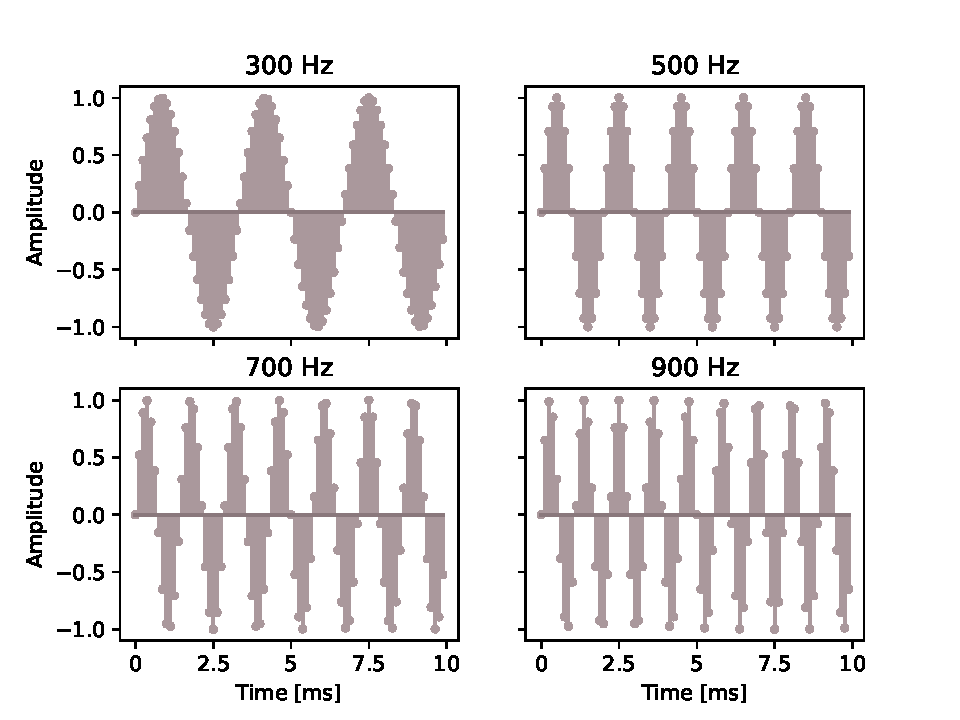
\includegraphics[width=0.85\textwidth]{figures/stem_300-500-700-900.pdf}
  \caption{Low Frequency Signals}\label{fig:low_freq_stem}
\end{figure}

\begin{figure}
  \centering
  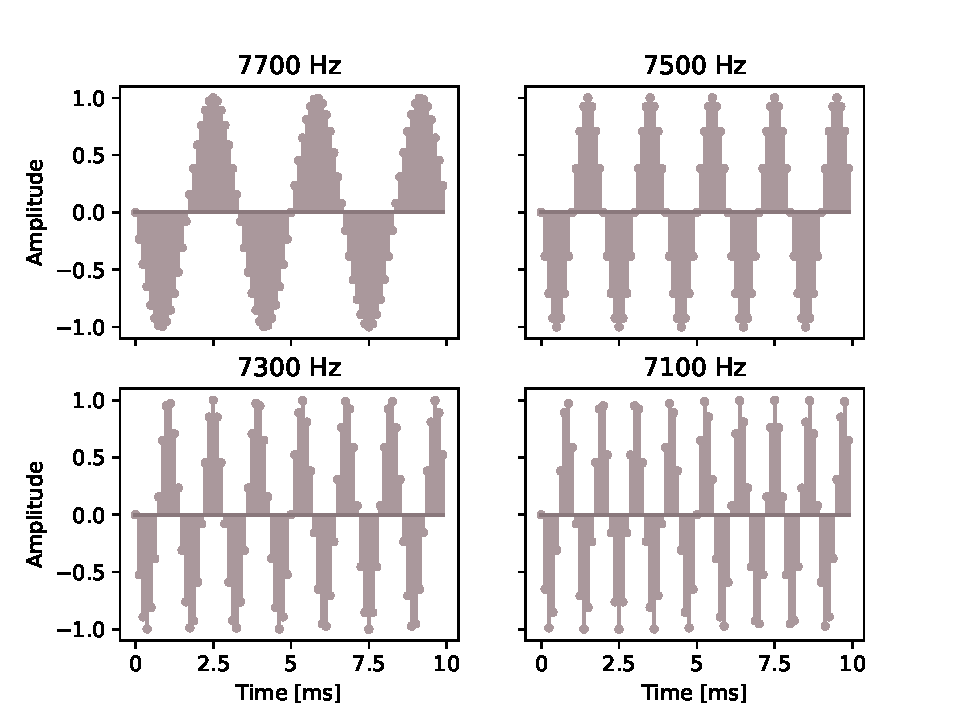
\includegraphics[width=0.85\textwidth]{figures/stem_7700-7500-7300-7100.pdf}
  \caption{High Frequency Signals}\label{fig:high_freq_stem}
\end{figure}

\begin{figure}
  \centering
  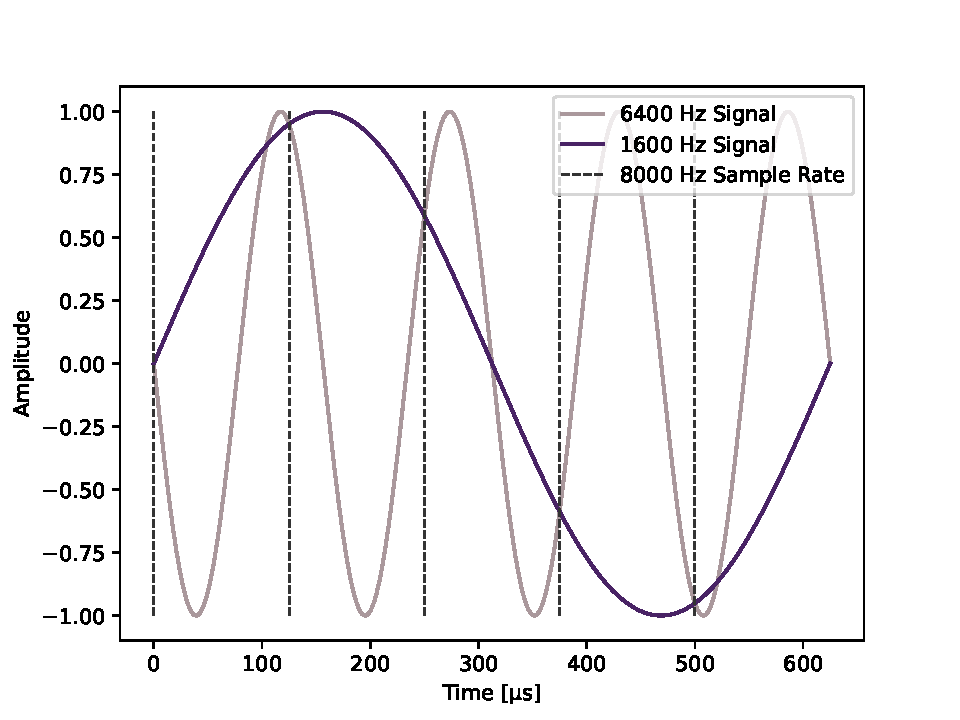
\includegraphics[width=0.75\textwidth]{figures/aliasing.pdf}
  \caption{Aliasing Demonstration}\label{fig:aliasing}
\end{figure}

\begin{figure}
  \centering
  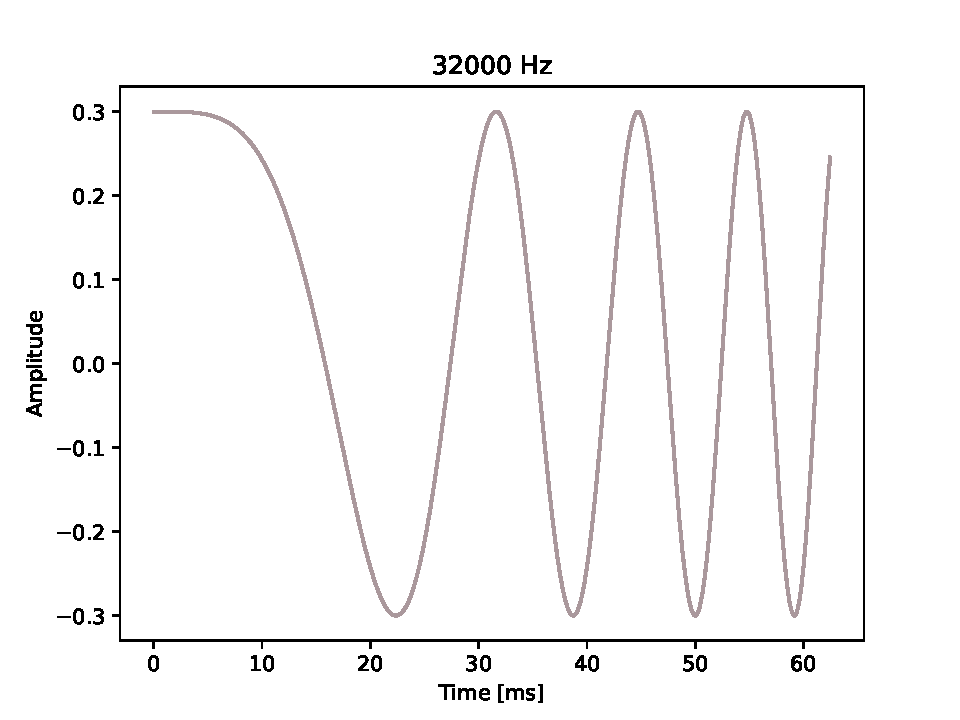
\includegraphics[width=0.75\textwidth]{figures/chirp_32000.pdf}
  \caption{Chirp Signal}
  \label{fig:chirp}
\end{figure}

\begin{figure}
  \centering
  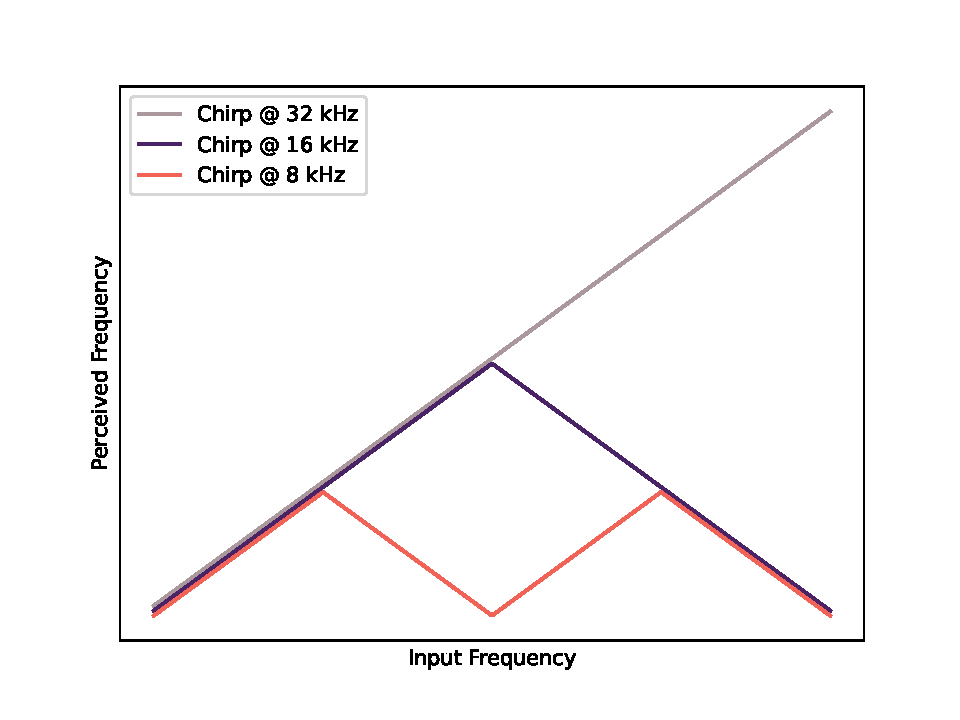
\includegraphics[width=0.75\textwidth]{figures/chirp_samples.pdf}
  \caption{Chirp Samples}
  \label{fig:chirp_samples}
\end{figure}

\end{document}
%%% Local Variables:
%%% mode: latex
%%% TeX-master: t
%%% End:
